\section{Anomaly Detection Data-Driven}

\subsection{Forecasting e Serie Temporali}

\subsubsection{Forecasting (SL)}

Nell'ambito del rilevamento delle anomalie basato sui dati
(Data Driven Anomaly Detection), un approccio fondamentale
è costituito dal ``\textbf{FORECASTING}'' o previsione.
Questa metodologia si basa sull'apprendimento supervisionato (SL)
e mira a identificare specifici descrittori all'interno delle
serie temporali. Tra questi descrittori, è cruciale distinguere
il \textbf{TREND}, che rappresenta l'andamento a lungo termine;
le \textbf{STAGIONALITÀ}, intese come ripetizioni periodiche;
e i \textbf{CICLI}, ovvero pattern simili che si ripetono con
periodicità variabile.

\begin{figure}[H]
    \centering
    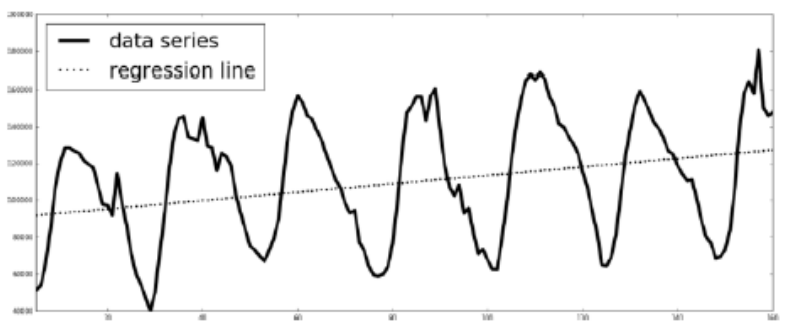
\includegraphics[width=0.8\textwidth]{img/forecasting.png}
\end{figure}

L'immagine mostra un grafico tipico
di una serie temporale, dove una linea continua (``data series'')
oscilla vistosamente evidenziando una stagionalità, mentre una
linea tratteggiata (``regression line'') attraversa il grafico
indicando la tendenza di crescita lineare sottostante (trend).
L'analisi di queste componenti permette di modellare il
comportamento atteso del sistema.

\subsubsection{Possible Approaches}

Per implementare sistemi di forecasting efficaci, si possono
adottare diversi approcci modellistici. Tra i metodi statistici
classici figurano i modelli autoregressivi, come \textbf{ARIMA},
mentre nel campo dell'apprendimento automatico avanzato si
utilizzano spesso reti neurali, in particolare le
\textbf{LSTM (Long Short-Term Memory)}, idonee per gestire
sequenze temporali lunghe.

\subsubsection{When Use Forecasting}

TUTTAVIA, è necessario valutare attentamente quando utilizzare
la previsione. Questa tecnica risulta appropriata principalmente
quando si analizza una metrica a valore singolo nel tempo.
È importante sottolineare che il forecasting non è intrinsecamente
adatto per il rilevamento degli outlier se il set di addestramento
contiene già delle anomalie. Infatti, se il training set è
``sporco'', il modello apprenderà sia i dati normali che quelli
anomali (outliers), compromettendo la capacità di rilevazione.
Questo metodo è quindi consigliato principalmente per identificare
anomalie che si verificano per la prima volta
(\textbf{first time anomaly}) o quando si dispone di un set di
addestramento pulito.

\begin{figure}[H]
    \centering
    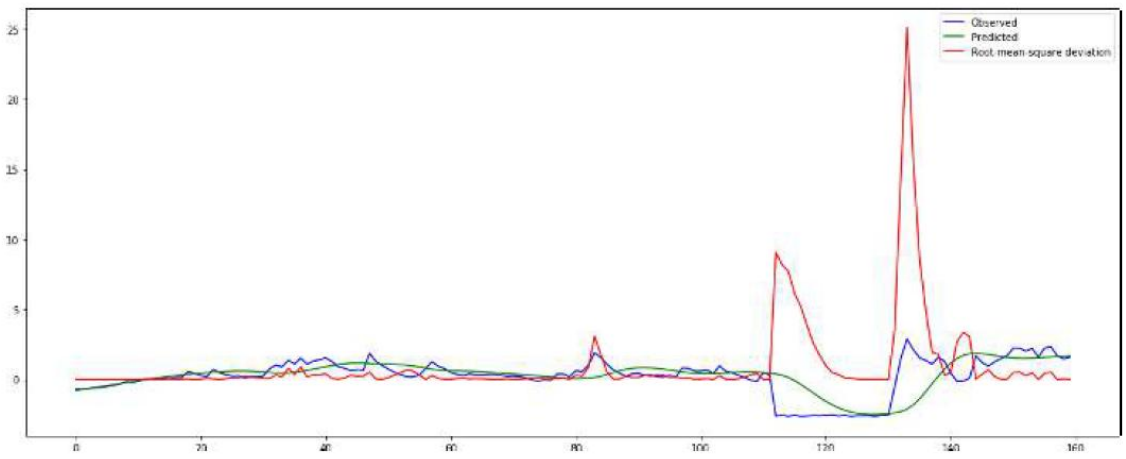
\includegraphics[width=0.8\textwidth]{img/anomaly.png}
\end{figure}

L'uso del forecasting è indicato solo quando emergono trend
osservabili con fluttuazioni limitate. In questo contesto,
le anomalie vengono rilevate analizzando la deviazione
quadratica media (\textbf{RMS deviation}). Il grafico
illustrativo mostra tre curve: i dati osservati, i dati
predetti e la deviazione RMS (linea rossa). Si nota chiaramente
un picco improvviso nella linea rossa in corrispondenza di un
evento anomalo, segnalando una discrepanza significativa tra
previsione e realtà.

\subsection{Metodi Statistici e Goodness-of-Fit}

\subsubsection{Statistical Methods}

Passando ai metodi statistici per il rilevamento delle anomalie,
una tecnica comune prevede il confronto della media mobile con
una soglia predefinita. Quando i dati vengono ridotti a un set
normale standard, i punti che risiedono nell'intervallo
$[-2, 2]$ sono generalmente considerati accettabili.
Un'alternativa più robusta è rappresentata dalla
\textbf{deviazione assoluta mediana (MAD - Median Absolute
Deviation)}. La MAD si calcola come la mediana delle deviazioni
assolute dalla mediana della serie:
\[
    MAD = \text{median}(|x - \text{median}(x)|)
\]
Poiché la mediana è statisticamente meno suscettibile della media
agli outlier, la MAD risulta essere una metrica particolarmente
robusta in dataset che prevedono valori anomali.

\subsubsection{Goodness-of-Fit}

I metodi statistici appena descritti presentano il vantaggio di
essere molto semplici. Quella semplicità si traduce in alta
spiegabilità (explainability) e riproducibilità dei risultati.
Inoltre, tali modelli sono facili da mantenere e da ottimizzare
(tuning). Tuttavia, la loro applicabilità è spesso limitata dalla
complessità dei dati reali.

Il concetto di ``\textbf{Bontà dell'adattamento}''
(\textbf{Goodness-of-fit}) prevede di confrontare la distribuzione
attesa derivante dal modello teorico con la distribuzione reale
osservata, al fine di rilevare anomalie. Nel mondo reale,
tuttavia, modellare dataset complessi utilizzando distribuzioni
semplici e note rappresenta una sfida significativa. Questo
approccio diventa fattibile e praticabile quasi esclusivamente
quando la distribuzione attesa è nota a priori.

\subsubsection{Known Tests (e.g. Chi-Squared Test)}

Tra i test statistici noti, il \textbf{test del chi-quadrato
($\chi^2$)} è uno dei più utilizzati, sebbene sia applicabile
principalmente a dataset unidimensionali, il che ne limita
l'applicabilità in contesti multi-dimensionali. Questo test si
basa sulla funzione di densità di probabilità del $\chi^2$
definita dalla formula che coinvolge i gradi di libertà ($k$),
la variabile casuale e la funzione GAMMA. I valori della
distribuzione $F(x, d)$ sono tabulati. Per applicare il test, è necessario definire un
livello di significatività $\alpha$ per valutare il valore
critico di confronto con il valore stimato, calcolato sommando
le differenze quadratiche normalizzate tra i valori osservati
($O_i$) e quelli attesi ($E_i$).

\subsection{Inviluppo Ellittico e Tecniche Non Supervisionate}

\subsubsection{Elliptic Envelope Fitting}

Quando si lavora con dati che seguono una distribuzione
Gaussiana, è possibile utilizzare il metodo dell'
\textbf{inviluppo ellittico (Elliptic Envelope)}.
Come mostrato nelle rappresentazioni grafiche, questo metodo
traccia delle ellissi concentriche attorno ai dati, che fungono
da curve di livello della densità di probabilità: i punti che
ricadono all'interno dell'ellisse centrale (zona grigia scura)
sono considerati ``inliers'' (dati normali), mentre i punti
esterni, distanti dal centro di distribuzione, sono classificati
come ``outliers'' (punti anomali).

L'approccio dell'inviluppo ellittico presenta tuttavia delle
limitazioni stringenti: è idoneo solamente per dataset distribuiti
normalmente. Inoltre, richiede di impostare a priori un rapporto
di outlier (guessing outlier ratio) per eliminare anomalie nei
dati di addestramento. Un altro aspetto critico è che la
dimensione temporale viene trascurata, sebbene il metodo possa
funzionare applicando finestre temporali.

\begin{figure}[H]
    \centering
    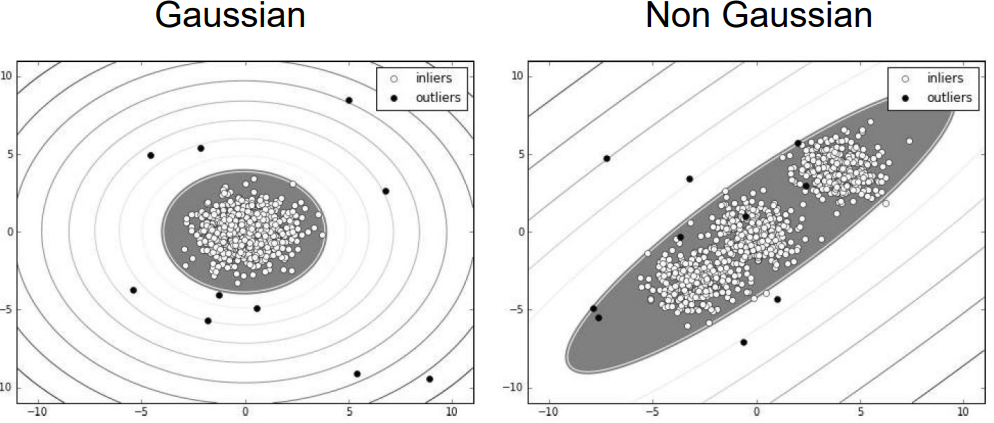
\includegraphics[width=0.8\textwidth]{img/elliptic.png}
\end{figure}

\subsubsection{Unsupervised Machine Learning (UL)}

Passando alle tecniche di apprendimento automatico non
supervisionato (Unsupervised Machine Learning - UL), troviamo
le \textbf{One-class SVM (Support Vector Machines)}. Questo
algoritmo addestra il modello adottando esclusivamente una
classe normale (traffico benigno). Di conseguenza, non possiede
un meccanismo di resistenza intrinseca, rendendo l'addestramento
meno resiliente agli outlier. Per tale motivo, le One-class SVM
sono più adatte per il rilevamento di novità
(novelty detection), come gli attacchi 0-day, piuttosto che
per il rilevamento di outlier, e funzionano al meglio se il
set di addestramento è stato preventivamente pulito dalle anomalie.

\subsection{Isolation Forests}

\subsubsection{Isolation Forests}

Le foreste di isolamento (Isolation Forests) rappresentano una
tecnica molto efficace che lavora bene con dataset ad alta
dimensionalità. Basandosi su strutture ad albero, risultano
computazionalmente efficienti. In questo modello, il numero
delle caratteristiche (feature) determina l'altezza dell'albero.

\subsubsection{Key Idea}

L'idea chiave alla base delle Isolation Forest è che le anomalie
possiedono un comportamento diverso rispetto al traffico normale
e, pertanto, possono essere isolate più facilmente all'interno di
un albero di ricerca. In termini pratici, ciò significa che
un'anomalia raggiungerà una foglia dell'albero con un numero
ridotto di salti (hops) o decisioni. L'immagine illustrativa
mostra come un punto ``facile da isolare'' (anomalia) si trovi
su un ramo corto vicino alla radice, mentre un punto ``difficile
da isolare'' (dato normale) richieda un percorso molto più lungo
attraverso le ramificazioni dell'albero.

\begin{figure}[H]
    \centering
    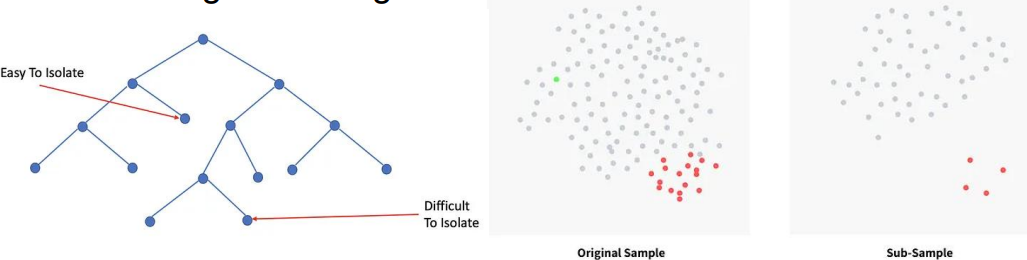
\includegraphics[width=0.8\textwidth]{img/isolationForest.png}
\end{figure}

\subsubsection{Additional Considerations}

Il traffico normale, essendo più omogeneo, tende a concentrarsi
nelle parti più profonde dell'albero. Una considerazione
importante riguarda la densità del dataset: un dataset meno
denso può aiutare a isolare le anomalie, in quanto diminuisce il
numero di campioni nella regione che separa i cluster di traffico
normale dai cluster di anomalie. Inoltre, non è necessario
costruire un albero completo per isolare le anomalie, poiché
tenderanno a risiedere vicino alla radice. Il sottocampionamento
(subsampling), mostrato graficamente nel confronto tra
``Original Sample'' e ``Subsample'', può favorire ulteriormente
l'isolamento delle anomalie riducendo il rumore.

\subsubsection{Costruzione e Punteggio di Anomalia}

Il processo prevede il campionamento del dataset $X$ per ottenere
un sottoinsieme $X_i$ con $\phi$ campioni, effettuato senza
reimmissione (without replacement). La dimensione raccomandata
per $\phi$ varia tra 128 e 512 elementi. L'altezza massima
dell'albero viene quindi impostata a $L = \log_2 \phi$.

\subsubsection{Average Tree Length}

Matematicamente, la lunghezza media del percorso di una ricerca
senza successo in un albero binario con $n$ nodi è data dalla
funzione:
\[
    c(n) = 2H(n-1) - \frac{2(n-1)}{n}
\]
dove $H(n)$ è il numero armonico stimato come
$\ln(n) + \gamma$ (costante di Eulero-Mascheroni). Questa formula
serve come base per la normalizzazione del punteggio di anomalia.
Per ogni sottoinsieme casuale, si costruisce un albero $T_i$
selezionando casualmente sia la caratteristica di divisione
(splitting feature) sia il punto di divisione.

\subsubsection{Evaluate the Anomaly Score}

Data una foresta composta da $n$ alberi casuali, per ogni
istanza $x$ nel set di test si valuta il numero di rami $h(x)$
attraversati dalla radice al nodo foglia nell'i-esimo albero.
Si calcola poi la media di questi valori su tutta la foresta,
ottenendo $E[h(x)]$. Il punteggio di anomalia $s(x, \phi)$
è definito come:
\[
    s(x, \phi) = 2^{-E[h(x)]/c(\phi)}
\]
L'interpretazione è la seguente: se la lunghezza media del
percorso $E[h(x)]$ è significativamente inferiore al costo medio
$c(\phi)$, allora $s$ tende a 1, indicando che $x$ è
un'anomalia. Se i valori sono molto vicini, non c'è evidenza
di anomalia (il punteggio tende a 0.5). Se la lunghezza del
percorso è maggiore del costo medio, il punteggio sarà molto
basso, indicando un dato normale.

\subsection{Metodi Basati sulla Densità e Local Outlier Factor}

\subsubsection{Density-Based Methods}

Passiamo ora ai metodi basati sulla densità. Questi includono
tecniche di clustering non supervisionato come il K-Means.
I metodi basati sulla densità sono particolarmente adatti per
dataset ad alta dimensionalità, situazioni difficili da gestire
con altre classi di metodi. L'idea principale è formare una
rappresentazione a cluster dei dati di addestramento, sotto
l'ipotesi che gli outlier o le anomalie si trovino nelle regioni
a bassa densità di questa rappresentazione. Tali approcci
risultano robusti agli outlier presenti nei dati di addestramento.

\subsubsection{Local Outlier Factor}

Anche variazioni dell'algoritmo K-NN possono essere utilizzate a
tale scopo, identificando i punti con elevata distanza dai
K-vicini più prossimi. Un approccio eccellente in questa
categoria è il \textbf{Local Outlier Factor (LOF)}.
Per ogni punto di test $A$, il LOF valuta la distanza di
raggiungibilità (reachability distance) dal K-vicino $B$,
definita come il massimo tra la distanza reale $d(A, B)$ e la
K-distanza di $B$. 

\begin{equation}
    d_k(A,B) = \max\{d(A,B),\ k\text{-}dist(B)\}
\end{equation}

Questa formulazione serve ad aumentare la
fluidità (smoothness) della misura. LOF valuta l'isolamento
di un punto rispetto alla densità dell'area circostante.

Successivamente, si valuta la densità di raggiungibilità
locale (local reachability density) di $A$ rispetto ai suoi
K-vicini. La LRD è calcolata come l'inverso della media delle
distanze di raggiungibilità sui vicini. Infine, il fattore LOF
si ottiene valutando il rapporto tra la LRD media dei vicini e
la LRD del punto $A$ stesso. 

\begin{equation}
    \mathrm{LRD}_k(A) = \left(\frac{1}{|N_k(A)|}
    \sum_{B \in N_k(A)} d_k(A,B)\right)^{-1}
\end{equation}

\begin{equation}
    \mathrm{LOF}_k(A) = \frac{1}{|N_k(A)|}
    \sum_{B \in N_k(A)} \frac{\mathrm{LRD}_k(B)}{\mathrm{LRD}_k(A)}
\end{equation}

L'interpretazione del rapporto è:
se il rapporto è minore o prossimo a 1, il punto $A$ ha una
densità simile ai suoi vicini ed è un inlier. Se il rapporto è
significativamente maggiore di 1 ($\gg 1$), significa che la
densità locale di $A$ è molto inferiore a quella dei suoi
vicini, identificandolo come un outlier.

\begin{figure}[H]
    \centering
    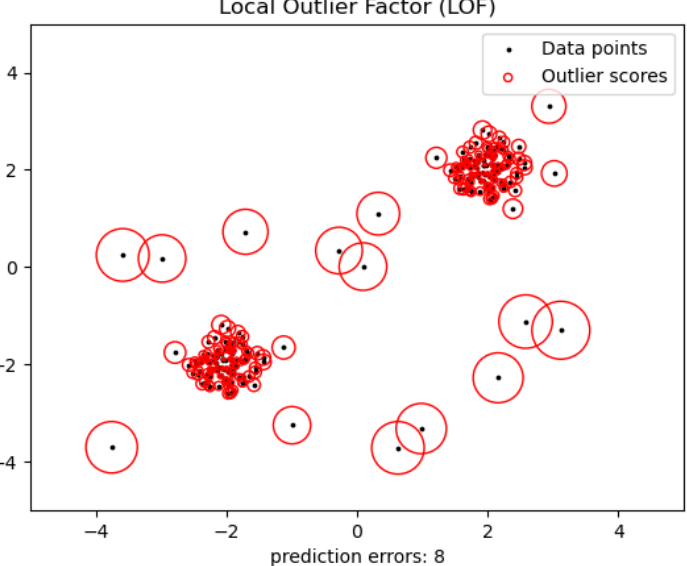
\includegraphics[width=0.5\textwidth]{img/density.png}
\end{figure}

Le immagini a supporto mostrano graficamente il concetto: punti
isolati hanno cerchi rossi più grandi che indicano punteggi
di outlier (LOF score) più elevati rispetto ai punti densamente
raggruppati nei cluster. Il LOF si basa esclusivamente sul
vicinato diretto e il punteggio è un rapporto derivante
principalmente dai suoi K vicini. Di conseguenza, la selezione
del valore $K$ risulta essere un parametro comune per il
successo dell'algoritmo.

\subsubsection{Selection of K-Value}

Per mitigare la sensibilità della scelta di $K$ è possibile
utilizzare una strategia di ensemble calcolando il punteggio
LOF con diversi valori di $K$. Generalmente, il valore minimo
di $K$ deve essere impostato a 10, mentre il massimo dipende
dai cluster dei dati. Tuttavia, questo metodo è generale può 
generare falsi positivi.
Sebbene rilevi sia anomalie locali che
globali, solitamente è utilizzato per le seconde. Inoltre, il metodo ha difficoltà a rilevare i bordi
di cluster vicini e richiede che i dati siano numerici e
varino continuamente.

\subsection{Autoencoder e Deep Learning per Anomalie}

Gli Autoencoder rappresentano un'importante applicazione delle
reti neurali del Deep Learning. Trovano ampio utilizzo in diversi
ambiti, tra cui la riduzione della dimensionalità, la compressione
delle immagini, la rimozione del rumore (denoising),
l'estrazione delle caratteristiche e, naturalmente, il
rilevamento delle anomalie.

\subsubsection{Autoencoder Structure}

Un Autoencoder (AE) è un tipo speciale di rete neurale profonda
progettata per copiare i valori di input nei valori di output.
In linea di principio, non richiede una variabile target come i
modelli standard, motivo per cui viene classificato come modello
non supervisionato. Il cuore dell'autoencoder è il livello
nascosto (hidden layer).

\begin{figure}[H]
    \centering
    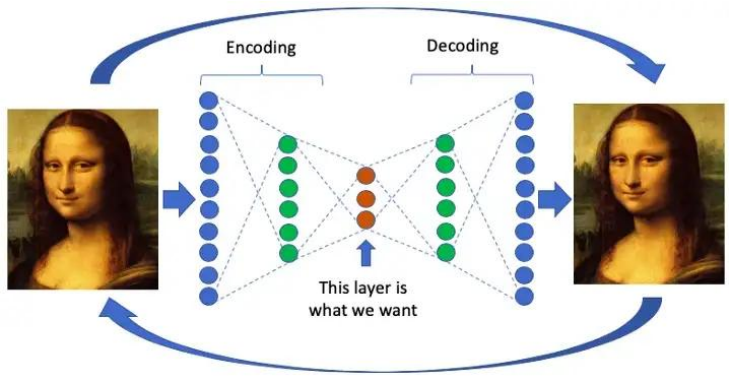
\includegraphics[width=0.7\textwidth]{img/autoencoders.png}
\end{figure}

\subsubsection{The Bottleneck Layer}

Quando il numero di neuroni negli strati nascosti è inferiore a
quello dei livelli di input, si crea un ``collo di bottiglia''
(bottleneck). Questa struttura forza i livelli nascosti a
estrarre le informazioni rilevanti e i pattern più rilevanti dei
dati ignorando il rumore. Pertanto, condizione necessaria in un
modello AE è che i livelli nascosti abbiano dimensioni minori
rispetto ai livelli di input e output.

\subsubsection{Encoding and Decoding}

Il funzionamento si articola in due processi: l'\textbf{encoding}
(codifica), che comprime i valori di input per arrivare al
livello centrale (con layer o rappresentazione latente), e il
\textbf{decoding} (decodifica), che ricostruisce l'info a partire
dalla rappresentazione compressa per produrre l'output.
La maggior parte dei praticanti adotta una simmetria strutturale
tra encoder e decoder. L'obiettivo ideale è che l'output
ricostruito $x'$ sia il più simile possibile all'input
originale $x$ ($x \approx x'$).

\subsubsection{Steps to Detect Anomalies}

L'immagine mostra lo schema di flusso:
Input $x$ $\rightarrow$ Encoder $\rightarrow$ Bottleneck
$\rightarrow$ Decoder $\rightarrow$ Output ricostruito $x'$.
Per utilizzare gli autoencoder nel rilevamento delle anomalie,
la procedura prevede di addestrare la rete fornendo in input
esclusivamente traffico normale (inclusi gli outlier). In questo
modo, il livello bottleneck apprenderà la rappresentazione
latente dei soli dati normali. Anche se classificato come non
supervisionato, non è problematico addestrarlo con traffico
normale poiché ne abbiamo solitamente in abbondanza, ma 
va riaddestrato spesso per riallinearlo.

\subsubsection{Reconstruction Error}

Il decoder cercherà l'output del bottleneck per ricostruire le
caratteristiche originali. Il passaggio logico è che una
immissione fraudolenta o un'anomalia sarà strutturalmente diversa
da una transazione normale. Poiché l'autoencoder ha imparato a
``minimizzare solo la normalità'', avrà difficoltà a ricostruire
il traffico d'attacco; di conseguenza, l'errore di ricostruzione
sarà elevato. L'input anomalo produrrà un output
significativamente diverso.

\subsubsection{MSE and Threshold}

Un evento viene segnalato come anomalia se il suo errore di
ricostruzione supera una certa soglia (threshold). Tale soglia
può essere definita valutando il k-esimo percentile della
funzione di perdita. In questo contesto, si utilizza tipicamente
l'\textbf{errore quadratico medio (MSE - Mean Square Error)}
per quantificare la distanza tra il campione originale $x$ e
quello ricostruito $x'$. La formula è la classica media delle
differenze al quadrato:
\[
    MSE = \frac{1}{N} \sum_{i} (x_i - x'_i)^2
\]
Si seleziona quindi un livello accettabile di falsi positivi per
determinare automaticamente la soglia: i campioni con $MSE > T$
saranno classificati come anomalie.

\begin{figure}[H]
    \centering
    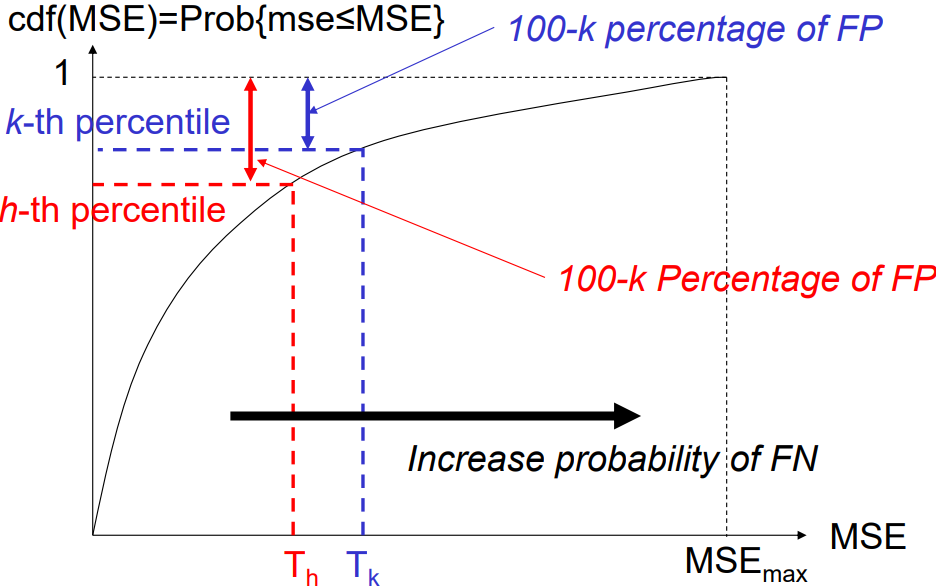
\includegraphics[width=0.7\textwidth]{img/MSE.png}
\end{figure}

\begin{figure}[H]
    \centering
    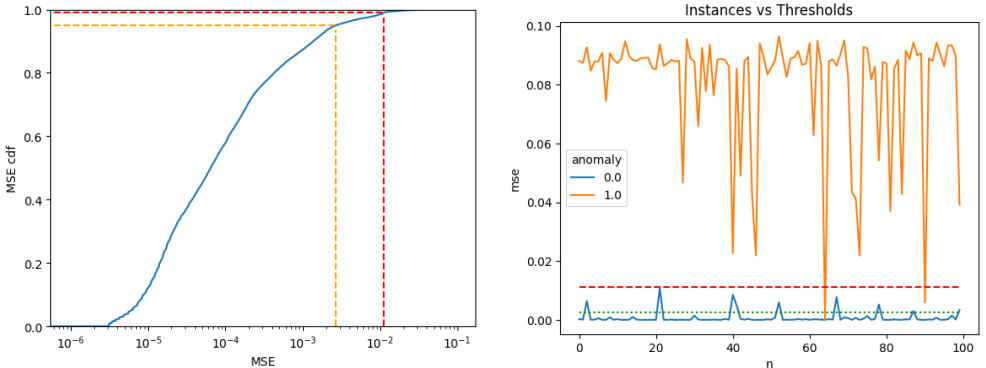
\includegraphics[width=0.8\textwidth]{img/MSE2.png}
\end{figure}

I grafici presenti aiutano a visualizzare la scelta della soglia.
Il primo grafico mostra la funzione di distribuzione cumulativa
(CDF) dell'MSE. Scegliendo un percentile (es. 95-esimo), si
determina una soglia $T_h$. Questo implica accettare una
percentuale $100 - k$ di falsi positivi. Aumentare la soglia
riduce i falsi positivi ma incrementa la probabilità di falsi
negativi. Il secondo grafico ``Instance vs Threshold'' mostra
l'MSE per diverse istanze: le anomalie (linee arancioni)
presentano picchi di errore (MSE) nettamente superiori alla
soglia (linea tratteggiata) rispetto ai dati normali
(linee blu) che rimangono bassi e stabili.

\subsubsection{Data Augmentation}

Concludiamo toccando alcuni argomenti avanzati.
La \textbf{data augmentation} (aumento dei dati) è cruciale
quando i dati sono sbilanciati. Esistono approcci ``anello
aperto'' (open loop) come la tecnica
\textbf{SMOTE (Synthetic Minority Oversampling Technique)}
e le sue varianti, che generano campioni sintetici della classe
minoritaria interpolando i dati esistenti. Parallelamente, vi
sono approcci a ``anello chiuso'' (closed loop) che utilizzano
reti avversarie (\textbf{GAN - Generative Adversarial Networks})
per creare dati sintetici realistici.

\subsubsection{Security and Feedback}

Infine, è doveroso menzionare le vulnerabilità di sicurezza dei
modelli di Machine Learning. Gli ``esempi avversari''
(adversarial examples) sono input appositamente perturbati per
ingannare e far fallire i modelli ML; per difendersi, si ricorre
all'addestramento avversario (adversarial training). Un'altra
frontiera è rappresentata dagli approcci basati sul feedback,
come l'\textbf{apprendimento per rinforzo (Reinforcement
Learning)}, dove il modello impara e si adatta interagendo
dinamicamente con l'ambiente.
